\chapter{氢与 s 区}\label{ch:b1:s-block}

每一部手机、笔记本电脑和电动汽车都装有电池，其
正电荷由锂离子携带。这种锂主要来自两处：
澳大利亚的硬岩矿山，以及安第斯山脉的盐沼。
在盐沼中，从地壳深处抽取的卤水被晾晒于阳光下蒸发，历时
数月，直至能从中沉淀出锂盐。锂是\omterm{def:b1:s-block:families}{碱金属}中的
第一个元素，也是现有金属中活性最强的。它的近邻
钠、钾、镁和钙，为工业提供大宗化学品：
烧碱、纯碱和石灰。本章以氢和 s 区开始
元素的描述性化学，
运用前几章的工具——电离能、
\omterm{def:b1:nernst:electrode-potential}{标准电极电势}、\omterm{def:b1:precipitation:solubility-product}{溶度积}——来解释这些
元素的行为。

\begin{recall}
电离能与\omterm{def:b1:periodicity:electronegativity}{电负性}（见\cref{ch:b1:periodicity}）；
\omterm{def:b1:nernst:electrode-potential}{标准电极电势}（见\cref{ch:b1:nernst}）；\omterm{def:b1:precipitation:solubility-product}{溶度积}与
氢氧化物的沉淀（见\cref{ch:b1:precipitation}）。第 1 册
（十年级）将元素分为若干族：\omterm{def:b1:s-block:families}{碱金属}、
\omterm{def:b1:s-block:families}{碱土金属}、卤素、稀有气体。
\end{recall}

\begin{omfigure}
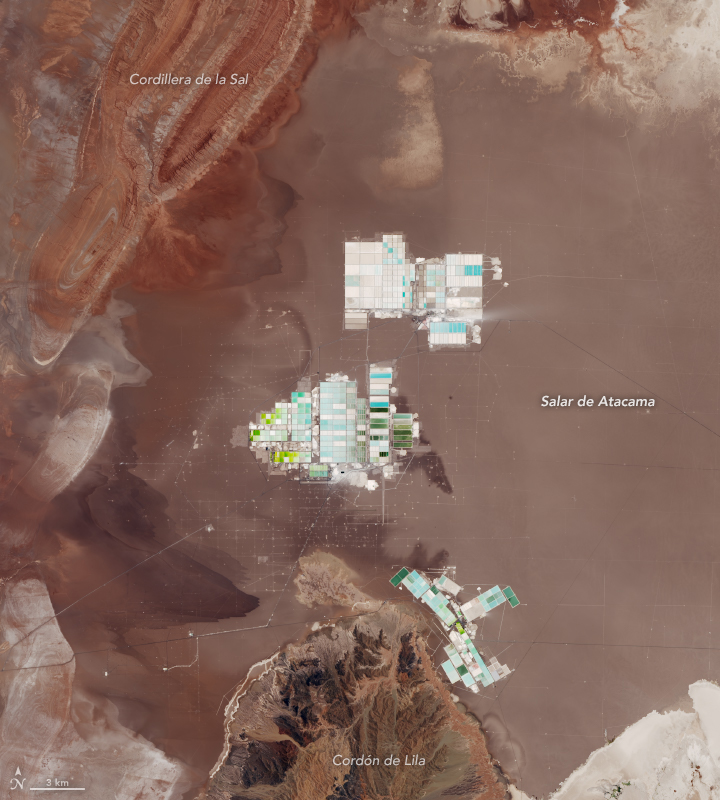
\includegraphics[width=0.48\linewidth]{images/book2/atacama-ponds.jpg}

{\small 阿塔卡马盐沼上的锂卤水蒸发池，
自轨道所见
（照片：Landsat 8，2018 年；NASA 地球观测站，公有领域，维基共享资源）。各池的颜色随卤水
浓缩和盐类结晶而变化。}
\end{omfigure}

\section{氢与氢化物}

氢原子只有一个电子：可以失去它（\ce{H+}，水中以
\ce{H3O+} 形式存在），可以共享（形成\omterm{def:b1:lewis-resonance-vsepr:lewis}{共价键}），或得到一个电子（\ce{H-}，
电子构型与氦相同）。具体采取哪种方式，取决于其结合对象。

\begin{definition}[氢化物]\label{def:b1:s-block:hydride}
称\emph{氢化物}\index{氢化物}为氢与另一种
元素组成的二元化合物。\emph{离子型氢化物}\index{离子型氢化物}，
与\omterm{def:b1:s-block:families}{碱金属}及较重的\omterm{def:b1:s-block:families}{碱土金属}形成（\ce{LiH}、\ce{NaH}、
\ce{CaH2}），是含 \ce{H-} 的离子型固体。\emph{共价型氢化物}\index{共价型氢化物}
与 p 区元素形成，
（\ce{CH4}、\ce{NH3}、\ce{H2O}、\ce{HCl}），为分子型。\emph{金属型氢化物}\index{金属型氢化物}
与部分过渡金属形成，为固体，
其中氢占据金属\omterm{def:b1:crystals-metals:lattice}{晶格}的
\omterm{def:b1:crystals-metals:site}{间隙位置}，组成往往可变。
\end{definition}

氢负离子是很强的碱和\omterm{def:b1:nernst:couple}{还原剂}。\omterm{def:b1:s-block:hydride}{离子型氢化物}
与水反应，\ce{NaH + H2O -> NaOH + H2}，可用作溶剂的干燥剂，
也可在有机合成中用作碱（见\cref{ch:b1:alcohol-activation}）。
第二\omterm{def:b1:periodicity:table}{周期}的\omterm{def:b1:s-block:hydride}{共价型氢化物}显示出\omterm{def:b1:periodicity:electronegativity}{电负性}
沿该\omterm{def:b1:periodicity:table}{周期}的变化趋势：\ce{CH4} 既非酸性也非碱性，\ce{NH3}
呈碱性，\ce{H2O} 呈两性，\ce{HF} 呈酸性。

\section{碱金属}

\begin{definition}[碱金属与碱土金属]\label{def:b1:s-block:families}
\emph{碱金属}\index{碱金属}（Li、Na、K、Rb、Cs、Fr）
构成第 1 族，具一个\omterm{def:b1:quantum-numbers:configuration}{价电子}（\textit{ns}$^1$）；\emph{碱土金属}\index{碱土金属}
（Be、Mg、Ca、Sr、Ba、Ra）构成第 2 族，
具两个\omterm{def:b1:quantum-numbers:configuration}{价电子}（\textit{ns}$^2$）。这些元素组成
s 区。
\end{definition}

\begin{proposition}[碱金属是强还原剂]\label{prop:b1:s-block:reducing-power}
\omterm{def:b1:s-block:families}{碱金属}的\omterm{def:b1:periodicity:ionisation-energy}{第一电离能}在各自\omterm{def:b1:periodicity:table}{周期}中最低
（Li \qty{5.39}{eV}，Na 5.14，K 4.34），\omterm{def:b1:nernst:electrode-potential}{标准电极电势}很负
（\ce{Li+}/\ce{Li} $-3.04$~V，\ce{Na+}/\ce{Na} $-2.71$，
\ce{K+}/\ce{K} $-2.94$）：它们能还原水，在自然界中仅以
\ce{M+} 离子形式存在。
\end{proposition}
% ledger: ie:Li, ie:Na, ie:K (E0 computed in figdata/bachelor-1/standard-potentials.py)

\begin{proof}
一个位于稀有气体原子实之外的单电子，离原子核较远，
且受\omterm{def:b1:quantum-numbers:configuration}{内层电子}屏蔽（见\cref{ch:b1:periodicity}），很容易
被移去。在水中，半径小的 \ce{M+} 离子水合作用强，这使
电对电势进一步降低。$E^\circ$ 比 pH 7 时
水的电势线（$-0.41$~V）低 \qty{2.2}{V} 以上，反应
\ce{2M + 2H2O -> 2M+ + 2OH- + H2} 的平衡常数极大
（见\cref{prop:b1:nernst:equilibrium-constant}）。
\end{proof}

\begin{omfigure}
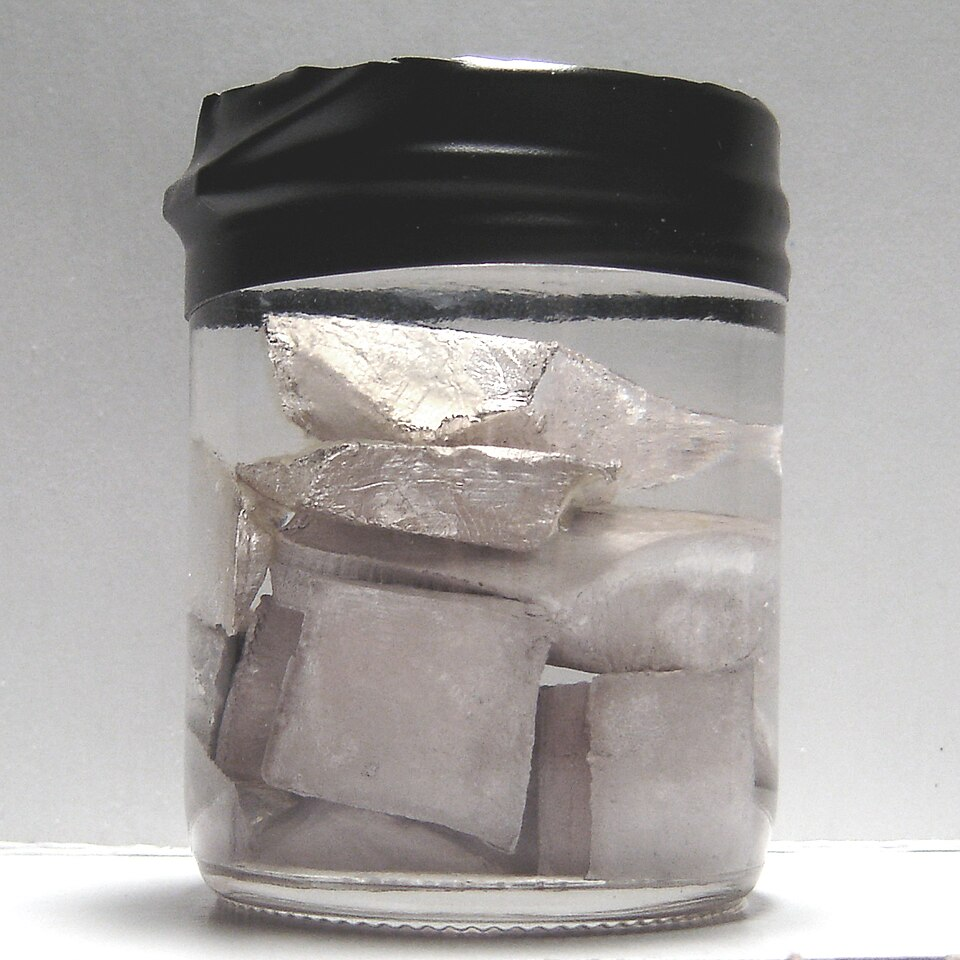
\includegraphics[height=4.6cm]{images/book2/sodium-oil.jpg}\hspace{0.8em}%
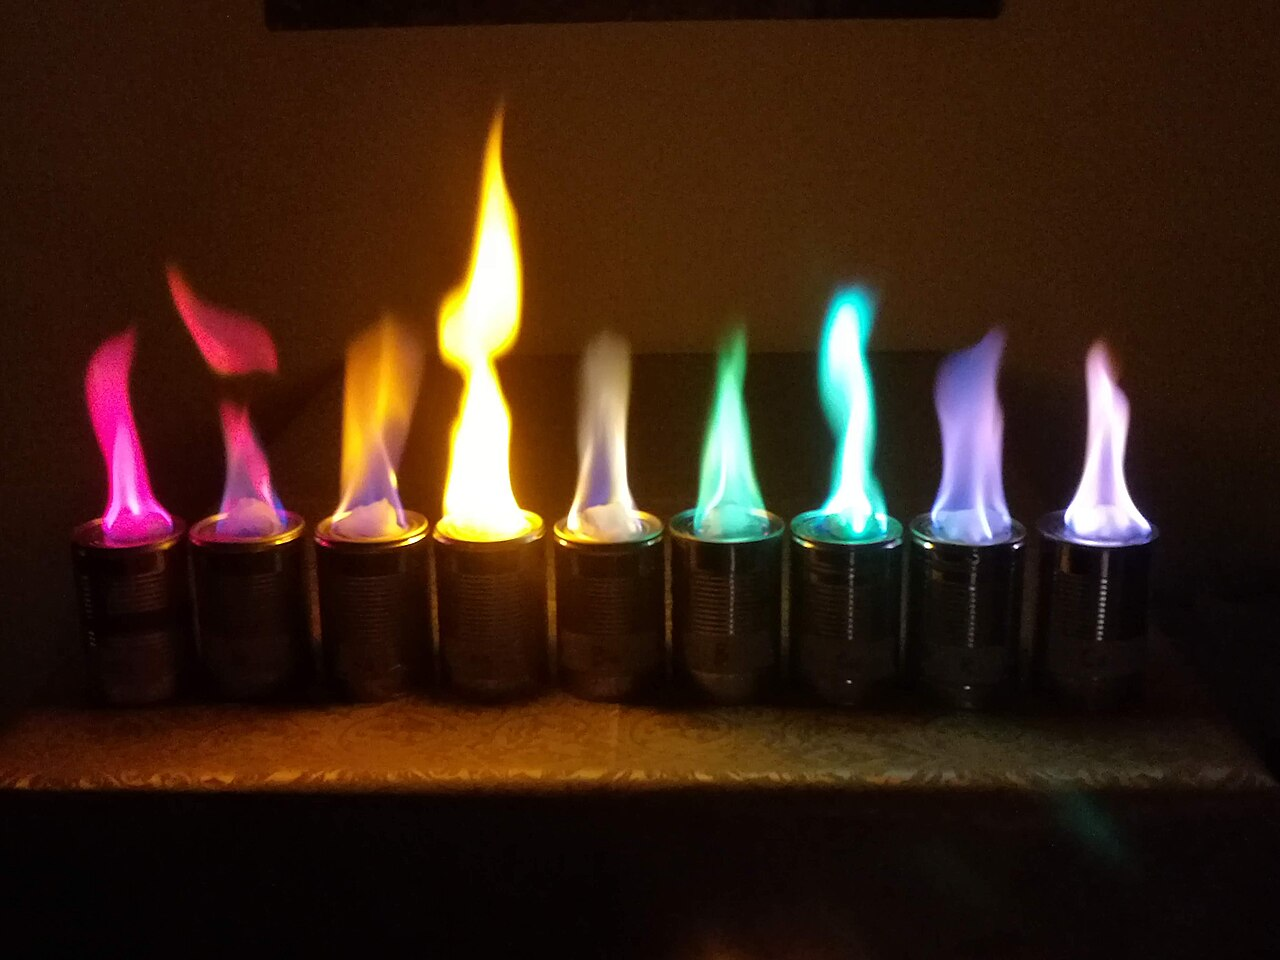
\includegraphics[height=4.6cm]{images/book2/flame-colours.jpg}

{\small 左：钠保存在矿物油中，以隔绝空气和水汽
（照片：Justin Urgitis，CC BY-SA 2.5）。右：焰色，自左至右
依次为锂、锶、钙、钠、钡、硼、铜、
铯和钾的化合物：火焰中受激的电子回到
较低\omterm{def:b1:quantum-numbers:energy-level}{能级}，并以各元素特有的波长发光
（见\cref{ch:b1:quantum-numbers}）（照片：Hegelrast，CC BY-SA 4.0）。两图均取自
维基共享资源。}
\end{omfigure}

\begin{inthelab}[演示，而非实验]
钠与水的反应仅由教师在安全屏后演示。
取一小块扁豆大小的钠投入装有酚酞的大水槽中，金属
熔化成一个运动的小球，氢气冒泡，粉红色的
痕迹表明生成了氢氧化物。钾会点燃氢气。
较大的块会爆炸。钠须在油下切割，用镊子夹取，
并以乙醇销毁残余物，
绝不可用水。
\end{inthelab}

锂是本族的例外：其离子最小、水合作用最强，
因而电势最负，但与水反应却最慢。其
化合物与镁的相似（碳酸锂和磷酸锂
与镁的一样微溶），两者在\omterm{def:b1:periodicity:table}{周期}表中处于
对角线关系。\omterm{def:b1:s-block:families}{碱金属}由其熔融氯化物电解制得，
因为没有足够强的化学\omterm{def:b1:nernst:couple}{还原剂}；
此类电池的电极反应，
在本科二年级分册中学习。

\section{钠的工业化合物}

\begin{definition}[氧化物的性质]\label{def:b1:s-block:oxide-character}
\emph{碱性氧化物}\index{碱性氧化物}与水反应生成
氢氧化物，或与酸反应生成盐（\ce{Na2O}、\ce{CaO}）；
\emph{酸性氧化物}\index{酸性氧化物}与水反应生成酸，
或与碱反应生成盐（\ce{CO2}、\ce{SO3}、\ce{P4O10}）；
\emph{两性氧化物}\index{两性氧化物}既能与酸反应，
又能与碱反应（\ce{Al2O3}、\ce{ZnO}）。同一\omterm{def:b1:periodicity:table}{周期}内，氧化物由碱性
（金属，左侧）逐渐过渡为酸性（非金属，右侧）。
\end{definition}

氢氧化钠由电解食盐水制得（即氯碱法，
同时得到氯气和氢气）。碳酸钠，即纯碱，
用于玻璃、洗涤剂及锂的提取，可以开采天然碱矿
，也可以由食盐和石灰石制得。2025 年，全球
产量约为 7100 万吨，其中 1900 万吨来自天然矿藏，
5200 万吨为人工合成，其中大部分采用索尔维法制得。
% ledger: usgs:sodaash-total-2025, usgs:sodaash-natural-2025, usgs:sodaash-synthetic-2025

\begin{proposition}[索尔维法]\label{prop:b1:s-block:solvay}
索尔维法将氯化钠和碳酸钙转化为
碳酸钠和氯化钙，\ce{2NaCl + CaCO3 -> Na2CO3 +
CaCl2}，过程中氨和二氧化碳循环使用。
\end{proposition}

\begin{proof}
各步骤为：(1) \ce{CaCO3 -> CaO + CO2}（石灰窑）；(2) \ce{NaCl + NH3 +
CO2 + H2O -> NaHCO3 + NH4Cl}（氨盐水的碳酸化；
其中\omterm{def:b1:precipitation:solubility}{溶解度}最小的盐碳酸氢钠沉淀析出）；(3)
\ce{2NaHCO3 -> Na2CO3 + CO2 + H2O}（煅烧）；(4) \ce{CaO + H2O ->
Ca(OH)2}；(5) \ce{Ca(OH)2 + 2NH4Cl -> CaCl2 + 2NH3 + 2H2O}（氨的
回收）。将 $(1) + 2\times(2) + (3) + (4) + (5)$ 相加，
\ce{NH3}、\ce{CO2}、\ce{NH4Cl}、\ce{NaHCO3}、\ce{CaO}、\ce{Ca(OH)2} 及水相互抵消：
\ce{2NaCl + CaCO3 -> Na2CO3 + CaCl2}。
\end{proof}

\begin{omfigure}
\begin{tikzpicture}[font=\small, >={Stealth}, box/.style={draw, rounded corners, fill=omDef!8, minimum width=2.6cm, minimum height=0.8cm, align=center}]
  \node[box] (kiln) at (0,0) {石灰窑 \\\ce{CaCO3 -> CaO + CO2}};
  \node[box] (tower) at (5.3,0) {碳酸化塔 \\\ce{NaHCO3} 析出};
  \node[box] (calc) at (10.2,0) {煅烧炉 \\\ce{NaHCO3} $\to$ \ce{Na2CO3}};
  \node[box] (slake) at (0,-2.6) {消化器 \\\ce{CaO + H2O -> Ca(OH)2}};
  \node[box] (still) at (5.3,-2.6) {氨蒸馏塔 \\\ce{NH4Cl + Ca(OH)2}};
  \draw[->, thick] (kiln) -- node[above] {\ce{CO2}} (tower);
  \draw[->, thick] (tower) -- node[above, font=\scriptsize] {固体 \ce{NaHCO3}} (calc);
  \draw[->, thick] (calc.north) -- ++(0,0.6) -| node[pos=0.25, above] {\ce{CO2} 循环} (tower.north);
  \draw[->, thick] (kiln) -- node[left] {生石灰 \ce{CaO}} (slake);
  \draw[->, thick] (slake) -- node[above, font=\scriptsize] {\ce{Ca(OH)2}} (still);
  \draw[->, thick] (tower) -- node[right] {\ce{NH4Cl}} (still);
  \draw[->, thick] (still.east) -- ++(1.2,0) |- node[pos=0.25, right] {\ce{NH3} 循环} ($(tower.east)+(0,-0.25)$);
  \draw[<-, thick] (tower.north west) -- ++(-0.5,0.6) node[above] {盐水 \ce{NaCl}};
  \draw[->, thick] (calc.east) -- ++(0.8,0) node[right] {\ce{Na2CO3}};
  \draw[->, thick] (still.south) -- ++(0,-0.6) node[below] {氯化钙 \ce{CaCl2}};
\end{tikzpicture}

{\small 索尔维法流程。二氧化碳和氨在循环中流动；
食盐和石灰石输入，纯碱和氯化钙输出。}
\end{omfigure}

\begin{omfigure}
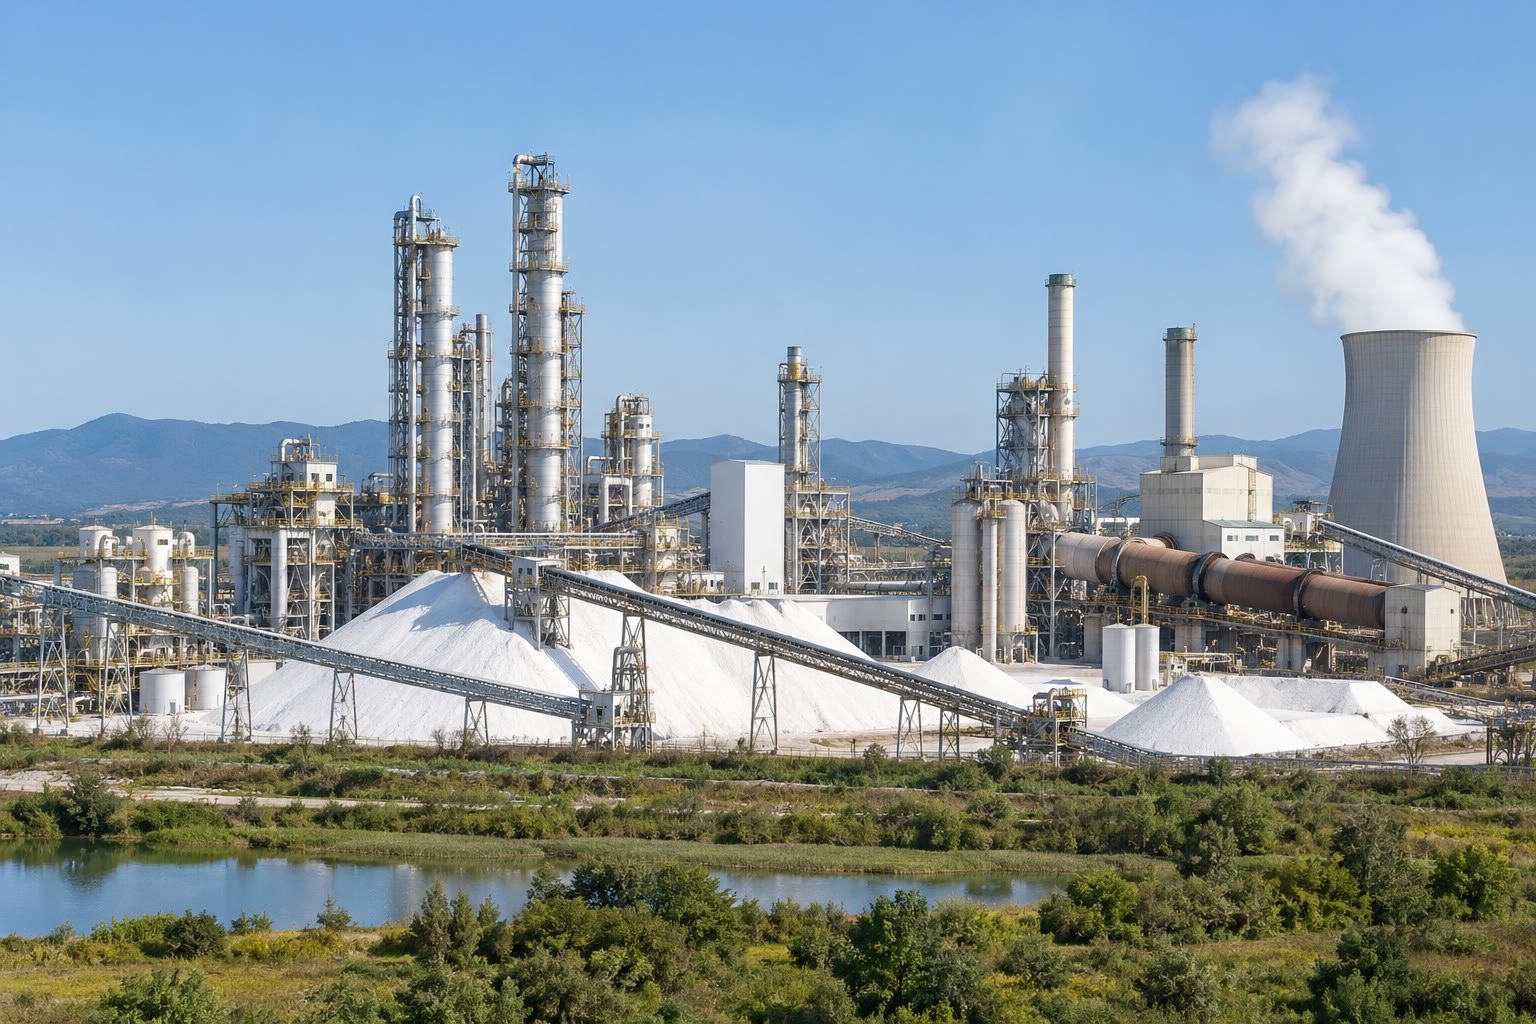
\includegraphics[width=0.55\linewidth]{images/book2/ai/b1-26-soda-ash-plant.jpg}

{\small 一座纯碱厂：石灰窑、碳酸化塔和堆放的
碳酸钠。}
\end{omfigure}

\begin{method}[流程图中的质量衡算]\label{met:b1:s-block:mass-balance}
\begin{enumerate}
  \item 写出总反应式（各步相加，循环物种
        相互抵消）。
  \item 由所需产物，用总反应式计算原料的用量，
        再按各步\omterm{def:b1:extent-q-and-k:fractional-extent}{产率}加以修正。
  \item 对于循环物种，只需计算
        补充其损失所需的量。
  \item 检查输入与输出之间每种元素的平衡。
\end{enumerate}
\end{method}

\section{碱土金属}

镁和钙的反应活性比\omterm{def:b1:s-block:families}{碱金属}低（
电离能较高：Mg \qty{7.65}{eV}，Ca 6.11；需失去两个电子），但
仍是较强的\omterm{def:b1:nernst:couple}{还原剂}（$E^\circ$（\ce{Mg^2+}/\ce{Mg}）为 $-2.36$~V）。
镁在空气中燃烧，发出耀眼的白光；其氧化膜
在室温下能保护镁。镁从海水中提取，方法是用石灰使其
氢氧化物沉淀，$\mathrm{p}K_s = 11.25$
（见\cref{ch:b1:precipitation}）。
% ledger: ie:Mg, ie:Ca

\begin{proposition}[石灰循环]\label{prop:b1:s-block:lime-cycle}
石灰石、生石灰、熟石灰与石灰石再次形成一个循环：
\ce{CaCO3 -> CaO + CO2}（窑中加热）；\ce{CaO + H2O -> Ca(OH)2}
（消化，强放热）；\ce{Ca(OH)2 + CO2 -> CaCO3 + H2O}（石灰
砂浆在空气中硬化）。整个循环在化学上没有净变化，
但会储存和释放能量及二氧化碳。
\end{proposition}

\begin{proof}
将三式相加，所有物种相互抵消。碳酸盐的分解
需要吸热，另外两步中又将热量放出；
窑中放出的 \ce{CO2} 又被砂浆缓慢吸收。
\end{proof}

\begin{omfigure}
\begin{tikzpicture}[font=\small, >={Stealth}]
  \node[draw, rounded corners, fill=omDef!8] (a) at (90:2.0) {\ce{CaCO3} 石灰石};
  \node[draw, rounded corners, fill=omDef!8] (b) at (-30:2.0) {\ce{CaO} 生石灰};
  \node[draw, rounded corners, fill=omDef!8] (c) at (210:2.0) {\ce{Ca(OH)2} 熟石灰};
  \draw[->, thick] (a) to[bend left=25] node[right, align=left] {加热 \\$-\ce{CO2}$} (b);
  \draw[->, thick] (b) to[bend left=25] node[below] {$+\ce{H2O}$} (c);
  \draw[->, thick] (c) to[bend left=25] node[left, align=right] {$+\ce{CO2}$\\$-\ce{H2O}$} (a);
\end{tikzpicture}

{\small 石灰循环：从石灰石到石灰砂浆，再回到
碳酸钙。}
\end{omfigure}

\section{锂}

\begin{omfigure}
\begin{tikzpicture}
\begin{axis}[
  xbar, width=0.78\linewidth, height=5.4cm, xmin=0, xmax=110,
  symbolic y coords={CA,ML,BR,AR,ZW,CL,CN,AU}, ytick=data,
  yticklabels={加拿大, 马里, 巴西, 阿根廷, 津巴布韦, 智利, 中国, 澳大利亚},
  xlabel={2025 年锂开采量（千吨 Li，估计值）}, bar width=8pt,
  nodes near coords, every node near coord/.append style={font=\scriptsize},
  tick label style={font=\small}, label style={font=\small}, enlarge y limits=0.1]
\addplot[fill=omDef!45, draw=omDef] coordinates {(5.6,CA) (9.4,ML) (12,BR) (23,AR) (28,ZW) (56,CL) (62,CN) (92,AU)};
\end{axis}
\end{tikzpicture}

{\small 2025 年主要锂生产国（估计值；全球总量
约 \num{290000} 吨锂）。澳大利亚开采硬岩
（锂辉石）；智利和阿根廷抽取卤水。}
% ledger: usgs:li-canada-2025, usgs:li-mali-2025, usgs:li-brazil-2025, usgs:li-argentina-2025, usgs:li-zimbabwe-2025, usgs:li-chile-2025, usgs:li-china-2025, usgs:li-australia-2025, usgs:li-world-2025
\end{omfigure}

卤水经蒸发浓缩，用石灰除去镁，
再用纯碱使碳酸锂沉淀。碳酸锂具有一种不寻常的性质：热时比冷时更难溶，
按质量计，\omterm{def:b1:precipitation:solubility}{溶解度}分别为 \qty{1.31}{\percent}（\qty{20}{\celsius}）、
\qty{0.84}{\percent}（\qty{80}{\celsius}）、
\qty{0.71}{\percent}（\qty{100}{\celsius}）。因此碳酸锂
应从热溶液中沉淀，如周末问题所计算的。
% ledger: sol:Li2CO3-20, sol:Li2CO3-80, sol:Li2CO3-100

\section{练习}

\begin{exercise}[$\star$]\label{exo:b1:s-block:1}
判断下列\omterm{def:b1:s-block:hydride}{氢化物}分别属于离子型、共价型还是金属型：\ce{KH}、\ce{SiH4}、
\ce{CaH2}、\ce{H2S}、\ce{PdH_{0.6}}。写出 \ce{CaH2} 与水反应的化学方程式。
\end{exercise}

\begin{exercise}[$\star$]\label{exo:b1:s-block:2}
写出锂、钠、钾分别与水反应，以及
镁与稀盐酸反应的化学方程式。
\end{exercise}

\begin{exercise}[$\star$]\label{exo:b1:s-block:3}
判断下列氧化物属于碱性、酸性还是\omterm{def:b1:s-block:oxide-character}{两性氧化物}：\ce{Na2O}、\ce{MgO}、\ce{Al2O3}、
\ce{SiO2}、\ce{SO3}、\ce{ZnO}、\ce{CO2}。每类各写出一个反应。
\end{exercise}

\begin{exercise}[$\star$]\label{exo:b1:s-block:4}
由\omterm{def:b1:nernst:electrode-potential}{标准电极电势}，计算反应 \ce{2Na + 2H2O -> 2Na+ + 2OH- + H2}
在 pH 14 时的平衡常数。
\end{exercise}

\begin{exercise}[$\star\star$]\label{exo:b1:s-block:5}
利用原子\omterm{def:b1:quantum-numbers:energy-level}{能级}，解释锂（红色）和钠（黄色）的
焰色（见\cref{ch:b1:quantum-numbers}）。求
波长为 \qty{589}{nm} 的黄色光子的能量。
\end{exercise}

\begin{exercise}[$\star\star$]\label{exo:b1:s-block:6}
计算用索尔维法制取一吨纯碱所需的石灰石（纯 \ce{CaCO3}）
与氯化钠的质量，已知以氯化钠计的总\omterm{def:b1:extent-q-and-k:fractional-extent}{产率}为
\qty{90}{\percent}。
\end{exercise}

\begin{exercise}[$\star\star$]\label{exo:b1:s-block:7}
海水中镁的含量约为 \qty{1.3}{g/L}（数据见本题）。
在何 pH 时氢氧化镁开始沉淀？
需多少质量的熟石灰才能使 \qty{1.0}{m^3} 海水中的镁沉淀？
\end{exercise}

\begin{exercise}[$\star\star$]\label{exo:b1:s-block:8}
尽管锂的\omterm{def:b1:nernst:electrode-potential}{标准电极电势}更低，为什么它与水的反应却比钾慢？
请区分热力学与动力学。
\end{exercise}

\begin{exercise}[$\star\star$]\label{exo:b1:s-block:9}
计算由一吨石灰石得到的生石灰质量，以及
在 \qty{25}{\celsius}、\qty{1}{bar} 下放出的 \ce{CO2} 体积。
\end{exercise}

\begin{exercise}[$\star\star\star$]\label{exo:b1:s-block:10}
2025 年全球约开采了 \num{290000} 吨锂。这些锂相当于
多少质量的碳酸锂？若一块汽车电池含 \qty{8}{kg} 锂
（数据见本题），则这些锂可供多少块此类电池使用？
\end{exercise}

\begin{exercise}[$\star\star\star$]\label{exo:b1:s-block:11}
由本章数据证明碳酸锂的\omterm{def:b1:precipitation:solubility}{溶解度}随温度升高而减小，
并解释为什么在热溶液中沉淀能提高
从卤水中的回收率。
\end{exercise}

\begin{exercise}[$\star\star\star$]\label{exo:b1:s-block:12}
在索尔维法的第 (2) 步中，溶液含有 \ce{Na+}、
\ce{NH4+}、\ce{Cl-} 和 \ce{HCO3-}。解释为什么碳酸氢钠
会沉淀而非氯化铵，以及为什么该过程
需要氨而非氢氧化钠。
\end{exercise}

\section{问题：从卤水中提锂}

\begin{problem}[{周末问题——浓缩锂卤水，
用石灰除镁，用纯碱沉淀碳酸锂，
并计算从一立方米中回收的碳酸锂质量}]
\label{pb:b1:s-block:1}
从盐湖地下抽取的卤水含锂 \qty{1.5}{g/L}，
含镁 \qty{0.60}{g/L}（以离子形式存在），并含大量氯化钠。
经蒸发池蒸发，卤水浓缩为原来的四倍。取一立方米该浓缩卤水
依次处理：用石灰除去镁，用纯碱除去钙，
最后以热纯碱在 \qty{80}{\celsius} 下使碳酸锂沉淀。
数据：摩尔质量（\unit{g/mol}）分别为 Li 6.9，Mg 24.3，
\ce{Ca(OH)2} 74.1，\ce{Na2CO3} 106.0，\ce{Li2CO3} 73.8；$\mathrm{p}K_s$
\ce{Mg(OH)2} 11.25，\ce{CaCO3} 8.30；$\mathrm{p}K_e = 14.00$；
\ce{Li2CO3} 在 \qty{80}{\celsius} 时的\omterm{def:b1:precipitation:solubility}{溶解度}（\omterm{def:b1:extent-q-and-k:composition}{质量分数}）为 \qty{0.84}{\percent}；
取最终母液为 \qty{1.00}{m^3}，密度为 \qty{1.0}{kg/L}。

\medskip
\noindent\textbf{第一部分——浓缩。}
\begin{enumerate}
  \item 计算浓缩卤水中锂和镁的
        浓度。
  \item 每立方米浓缩卤水需蒸发掉
        多少体积的水？
  \item 为什么采用太阳能蒸发而不是加热？
  \item 池中哪种盐先结晶析出？为什么？
  \item 计算一立方米卤水中锂和镁的物质的量。
  \item 为什么在沉淀锂之前必须先除去镁？
\end{enumerate}

\medskip
\noindent\textbf{第二部分——除去镁和钙。}
\begin{enumerate}[resume]
  \item 写出镁离子与熟石灰反应的方程式。
  \item 计算所需熟石灰的质量（按化学计量）。
  \item 溶液的 pH 为多少时，\qty{99.9}{\percent} 的镁被沉淀？
  \item 为什么锂不以氢氧化物的形式沉淀？
  \item 写出用纯碱除去引入的钙的反应。
  \item 计算该步骤所需纯碱的质量。
\end{enumerate}

\medskip
\noindent\textbf{第三部分——碳酸锂。}
\begin{enumerate}[resume]
  \item 写出碳酸锂沉淀的反应。
  \item 计算沉淀锂所需纯碱的质量。
  \item 计算碳酸锂的理论质量。
  \item 为什么沉淀要在 \qty{80}{\celsius} 下进行？
  \item 母液中仍溶解有多少质量的碳酸锂？
  \item 如何洗涤沉淀，才能使其损失尽量少？
\end{enumerate}

\medskip
\noindent\textbf{第四部分——物料衡算。}
\begin{enumerate}[resume]
  \item 计算回收的碳酸锂的质量。
  \item 计算锂的回收率。
  \item 说明母液如何处理。
  \item 将一立方米浓缩卤水中的锂与
        2025 年全球产量相比：该产量相当于多少立方米的卤水？
  \item 写出每立方米浓缩卤水
        所回收碳酸锂的质量。
\end{enumerate}
\end{problem}
